\section{Proposed Methodology}

\subsection{Queue-Centric Vision-Proxy Reward}
\label{sec:reward}
A central contribution of this work is the formulation of a reward function that is
strictly computable from camera-derived proxies, ensuring that the objective optimized
during simulation coincides with the metric available at deployment. The governing design
rule is that every reward term $r^{(k)}_i(t)$ factors through the vision-proxy projection
$\phi(\mathbf{s}_t)$ introduced in Section~\ref{sec:projection}. Unlike prior vision-based reinforcement
learning, which pairs a camera-constrained state with a privileged simulator reward
(typically the exact accumulated delay), no term in the proposed reward reads a privileged
quantity---the accumulated-delay penalty included, which is realized through a
halted-queue proxy. The objective is therefore deployable by construction.

The proposed reward $R_i(t)$ for intersection $i$ is a \emph{queue-centric} objective---a
congestion-minimization core, regularized by a throughput term and a switching term---written
as a weighted sum of six terms:
\begin{equation}
\begin{aligned}
R_i(t)
=&\;
w_q \frac{1}{n_i}\sum_{l=1}^{n_i} q_l^2
+w_p\, p_i(t)
+w_T\, T_i(t) \\
&+
w_s\, \mathbb{1}_{[\text{switch}]}
+w_v \max(\tau-\bar{v},0)
+w_w\, \bar{w}(t),
\end{aligned}
\label{eq:reward}
\end{equation}
where the weights are empirically set to
$w_q=-1.0$,
$w_p=-0.5$,
$w_T=+1.0$,
$w_s=-0.1$,
$w_v=-0.2$,
and
$w_w=-0.3$.
To ensure stable temporal-difference learning, the final scalar is clipped to
$[-2.0,\, +1.5]$. The individual components are detailed below.

These six terms are \emph{not} six orthogonal objectives: four are monotone functions of a
single congestion signal, the per-lane halted-queue fraction $q_l$
(\texttt{effective\_queue\_norm}). The queue penalty applies its $L_2$ norm
($\frac{1}{n_i}\sum_l q_l^2$, the Jensen anti-starvation form below); the accumulated-delay
penalty $\bar{w}(t)$ applies the $L_1$ norm of the \emph{same} vector---no per-vehicle
waiting timer is ever read, so in code it reduces exactly to the mean halted-queue
fraction, supplying a dense low-queue gradient that complements the quadratic term; the
low-speed penalty activates only when the mean approach speed $\bar{v}$ falls below the
threshold $\tau$, targeting stop-and-go congestion; and the phase-imbalance pressure rises
with the same congestion state. The two genuinely distinct regularizers are the local
ROI-exit throughput reward and the phase-switch penalty, the latter suppressing
high-frequency phase flickering. The reward is therefore dense, multi-scale gradient
shaping around a queue-minimization core, and the marginal value of each term
\emph{beyond} the $L_2$ core---rather than an assumption of independence---is what the
ablations of Section~\ref{sec:ablations} quantify.

\paragraph{Anti-starvation queue penalty}
Rather than the linear mean queue over the $n_i$ controlled lanes, the mean of
\emph{squared} queues $\frac{1}{n_i}\sum_{l=1}^{n_i} q_l^2$ is penalized. By Jensen's
inequality this exceeds the squared mean by exactly the per-lane queue variance, so the
quadratic form penalizes spatial imbalance at equal total demand and thereby discourages
the starvation of minor approaches.

\paragraph{Phase-imbalance pressure}
A signed \emph{phase-imbalance} term $p_i(t) \in [-1, 1]$ measures the queue delta between the
two fixed phase groups at the \emph{same} junction, partitioned by the currently red and green
movements:
\begin{equation}
p_i(t) = \frac{1}{n_i} \left( \sum_{l \in \text{red}} q_l - \sum_{l \in \text{green}} q_l \right).
\label{eq:pressure}
\end{equation}
This is an \emph{intra-junction} demand-imbalance gradient and is explicitly \emph{not} the
upstream--downstream network pressure of classical max-pressure
control~\cite{varaiya2013_maxpressure}; accordingly we do not claim the throughput-optimality
guarantee of max-pressure routing, and---compounded by per-lane normalization and value
clipping---the term functions as a highly reactive local heuristic rather than an optimal
routing policy. In contrast to a one-sided $\max(p, 0)$ surrogate, which provides zero gradient
whenever the active allocation is already correct, the signed form supplies a continuous
gradient that rewards serving the more congested group and penalizes serving the emptier one.

A naming subtlety: the reward pressure $p_i(t)$ is \emph{signal-relative}---evaluated
over the dynamic red/green partition induced by the active phase---whereas the
observation feature $\mathrm{pressure\_norm}$ of Section~\ref{sec:obs_space} is
\emph{geometry-relative}, encoding the static group-mean imbalance over the fixed groups
$A, B$. The phase one-hot identifies which fixed group holds green and
$\bar{q}_A - \bar{q}_B = 2\,\mathrm{pressure\_norm} - 1$, so the reward pressure is an
affine, phase-determined transform of observed quantities (exact up to approach
aggregation, equal-group scaling, and boundary saturation): the actor observes the
information its pressure reward optimizes.

\paragraph{Local ROI-exit throughput}
The agent is rewarded for vehicles actively clearing the intersection. The throughput term
is defined as
\begin{equation}
T_i(t) = \mathrm{clip}\!\left(\frac{1}{\kappa}\sum_{l \in L_i}\bigl|\, \text{prev\_ids}(l) \setminus \text{cur\_ids}(l)\, \bigr|,\; 0,\; 1\right),
\label{eq:throughput}
\end{equation}
with normalizing capacity $\kappa = 20$ and $L_i$ the set of lanes controlled by agent $i$.
Crucially, the simulator computation---the set difference of per-lane vehicle identities
between consecutive steps in SUMO~\cite{lopez2018_sumo}---is \emph{semantically identical}
to the deployable measurement of track identities terminating at the boundary of a
ByteTrack~\cite{zhang2022_bytetrack} region of interest (ROI). The reward signal is thus a
deployable metric in itself, incurring no domain shift. Because an exit is registered for
any identity present at the previous step and absent at the current one, lateral lane
changes (frequent under the sublane model) and the rare SUMO teleport are also counted as
exits; this is a bounded source of measurement noise that the deployable ByteTrack ROI-exit
counter shares identically, and therefore introduces no train/deploy discrepancy.

\subsection{MAPPO Architecture and Optimization}
\begin{figure*}[!t]
\centering
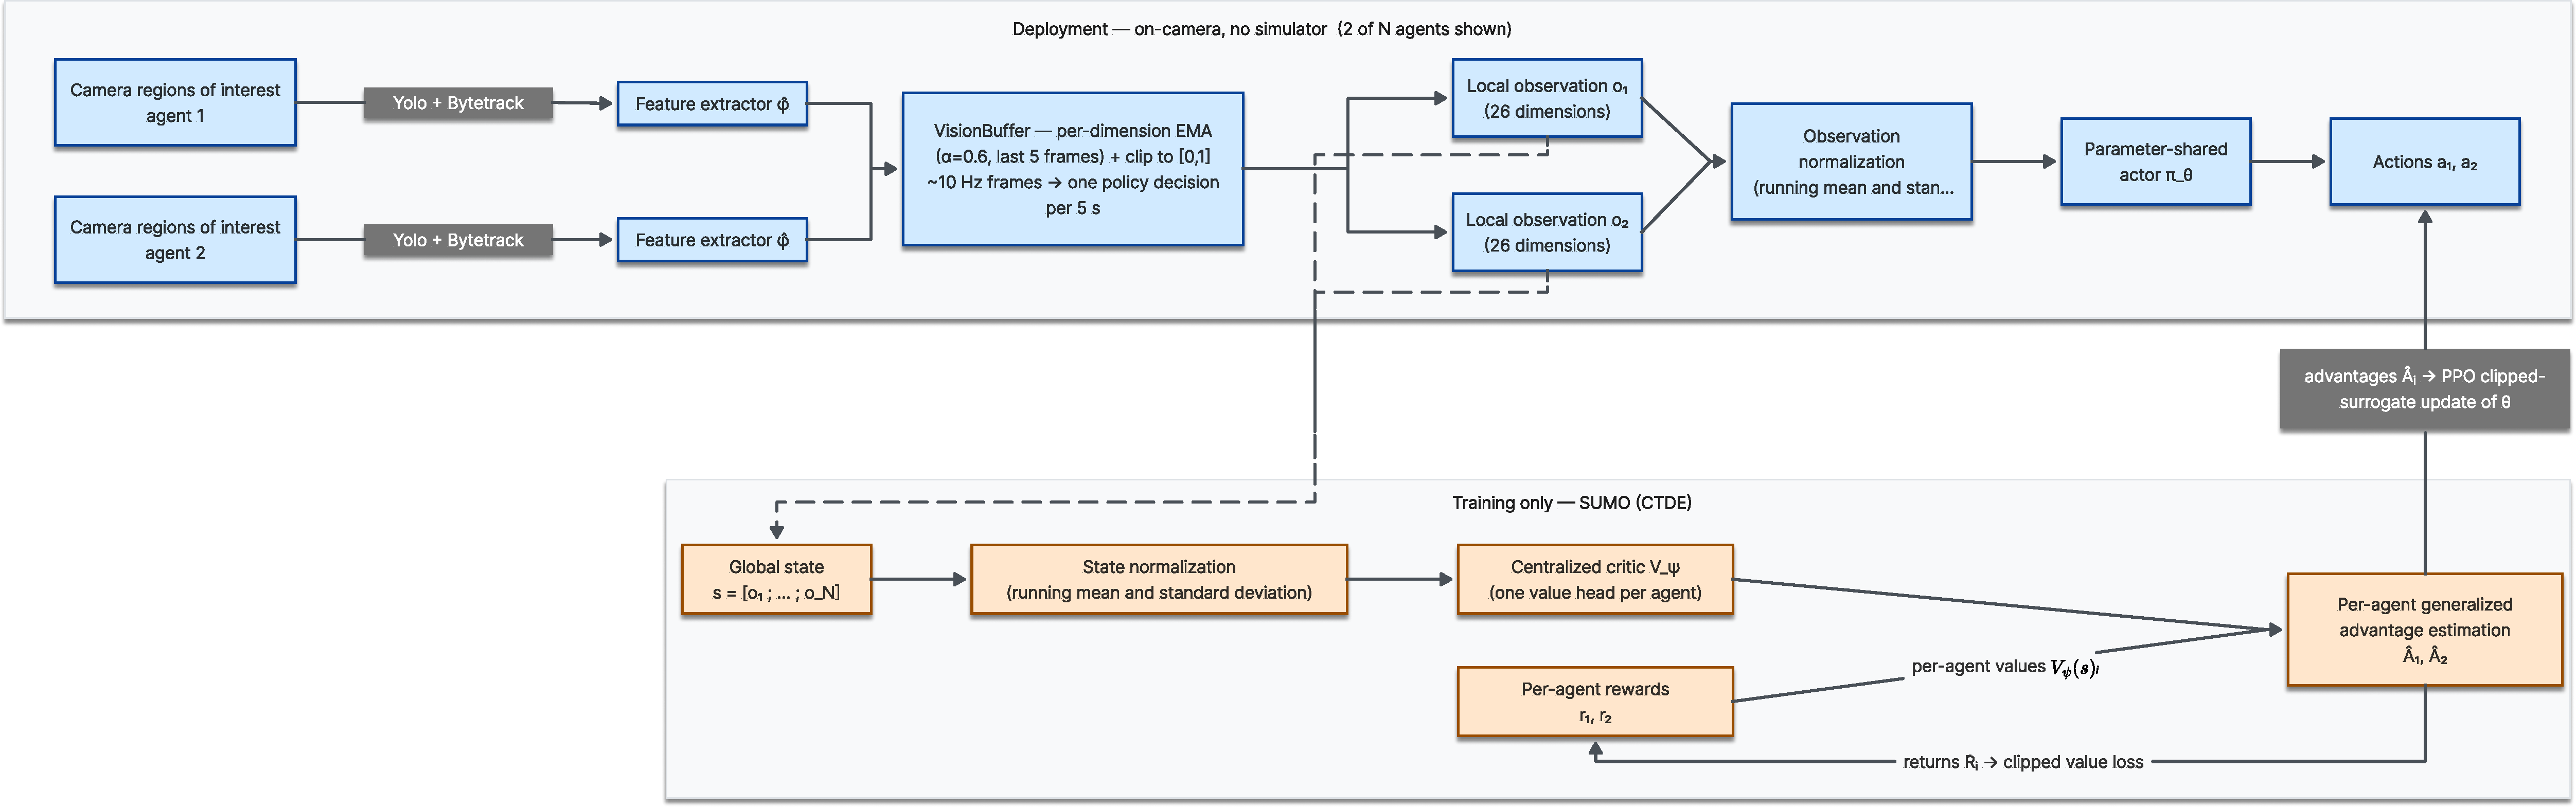
\includegraphics[width=\textwidth]{assets/figures/system_architecture.pdf}
\caption{Overall architecture of the proposed camera-observable multi-agent control
framework. Solid paths denote the on-camera deployment data flow (no simulator): per-agent
regions of interest are processed by YOLOv11 and ByteTrack, smoothed by a per-dimension
VisionBuffer (EMA, $\alpha=0.6$), normalized by the serialized Welford statistics, and
mapped to discrete phase actions by the parameter-shared actor $\pi_\theta$. Dashed paths
denote the training-only centralized multi-head critic and the per-agent GAE
estimator, neither of which is deployed.}
\label{fig:architecture}
\vspace{-4mm}
\end{figure*}

To optimize the multi-agent control policy, Multi-Agent Proximal Policy Optimization
(MAPPO)~\cite{yu2022_mappo} is adopted---a standard instance of the Centralized Training
with Decentralized Execution (CTDE) paradigm for the Dec-POMDP~\cite{oliehoek2016_decpomdp}
formalized in Section~\ref{sec:problem}. It is emphasized that the reinforcement-learning architecture
itself is standard and is not claimed as a methodological contribution; rather, it serves
as the vehicle through which the proposed camera-constrained state and vision-proxy reward
are evaluated.

The framework comprises a parameter-shared actor $\pi_\theta(a_{i,t}\,|\,\mathbf{o}_{i,t})$
that operates on the $26$-dimensional local proxy observation, yielding homogeneous control
behavior across intersections and facilitating zero-shot transfer to unseen topologies.
During training, a centralized critic $V_\psi(\mathbf{s}_t)$ ingests the concatenated global
proxy state. To preserve agent-specific reward shaping, the critic employs a multi-head
architecture that emits one value estimate per agent; this distinguishes the method from
the independent-critic IPPO~\cite{dewitt2020_ippo} baseline, in which each agent estimates
value from its local observation alone. Coordination in this design is achieved
\emph{solely} through the centralized critic: the per-agent rewards $r_{i,t}$ are strictly
local---each agent is credited only for the queues, phase imbalance, and ROI exits on its own
approaches, matching the deployment camera's field of view---so no inter-agent term appears in
the reward itself. Cross-intersection credit assignment enters only via the concatenated global
state ingested by the critic during centralized training and is absent at decentralized
execution, consistent both with the CTDE paradigm and with the camera-only constraint on the
deployed actor. Advantages $\hat{A}_{i,t}$ are computed via per-agent Generalized Advantage Estimation
(GAE)~\cite{schulman2016_gae} on the decentralized reward streams and standardized across all
agents within the batch. The actor and critic are then optimized using the standard PPO clipped
surrogate objective and a clipped multi-head value loss, respectively~\cite{schulman2017_ppo},
with early stopping triggered if the approximate KL divergence exceeds $1.5\times$ the target.

To bridge the residual normalization gap between training and deployment, the observation
running mean and variance are tracked online by Welford's algorithm~\cite{welford1962} and
serialized directly into the deployment checkpoint alongside the actor weights. Test-time
inputs $\mathbf{o}_{i,t}$ are therefore normalized with statistics identical to those seen
during training, without any dependence on live estimation.